% 钢结构论文图件插入片段
% 建议将 figures 文件夹上传至 Overleaf 项目根目录。
% 导言区需要：\usepackage{graphicx}

% 图1：装配式钢结构建筑技术体系图
% 建议插入章节：发展背景或技术特点
% 正文引用提示：如图~\ref{fig:01-technology-system} 所示，用于说明装配式钢结构由设计、制造、运输、安装、运维多环节协同构成。
\begin{figure}[htbp]
  \centering
  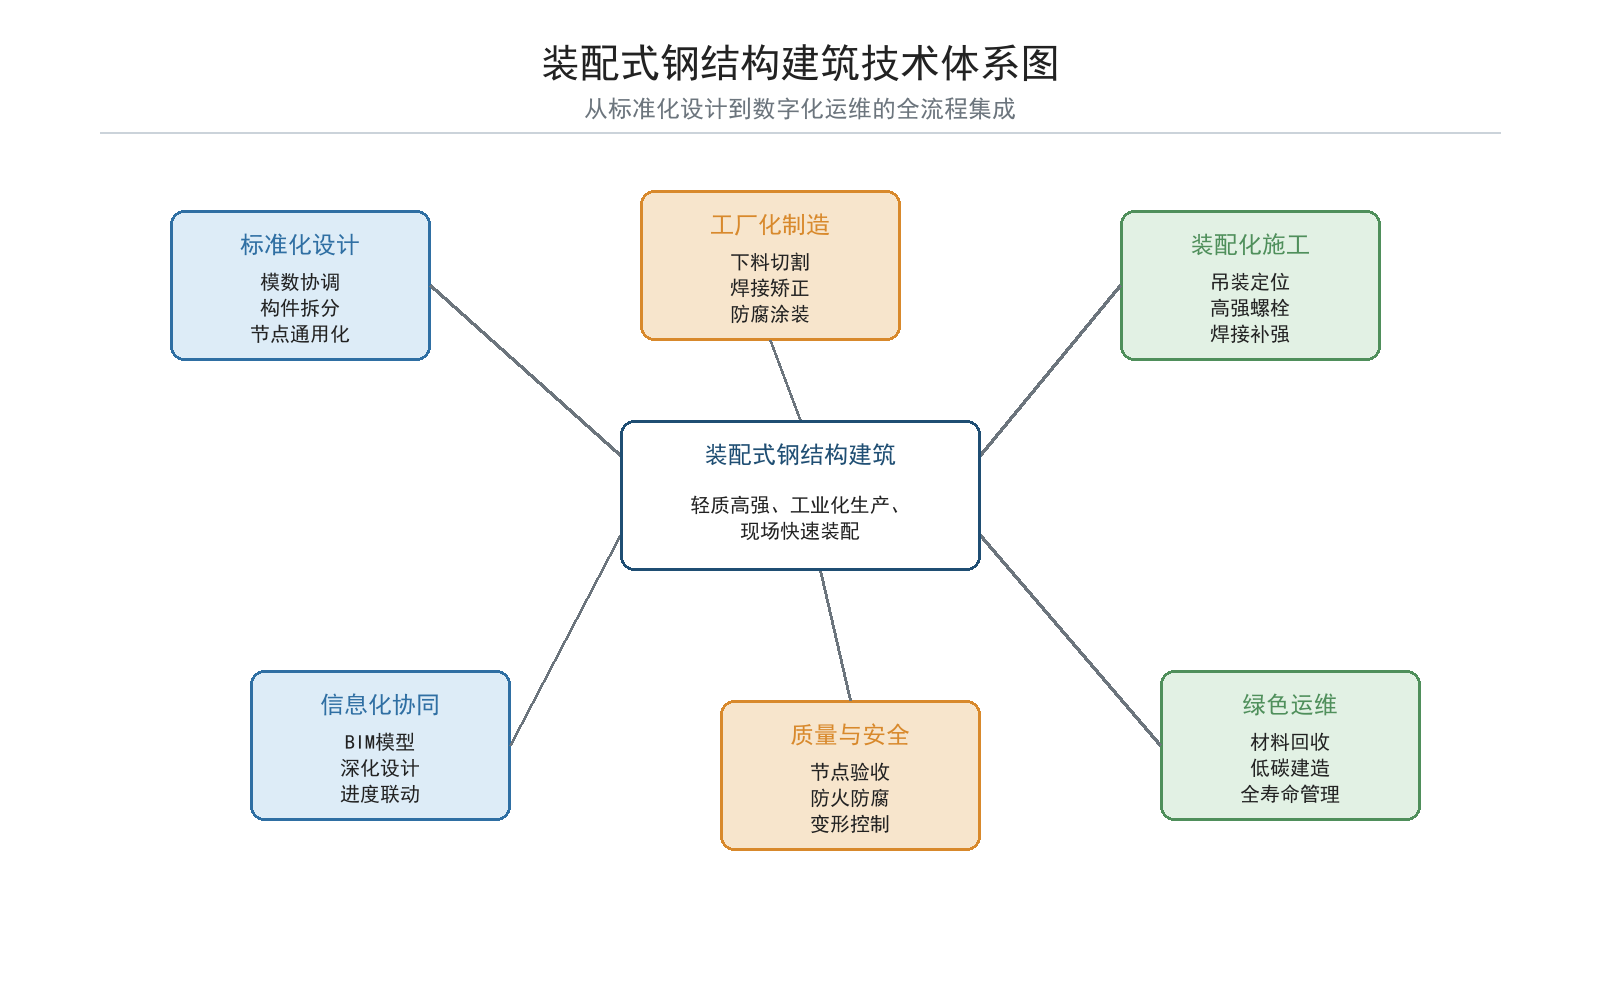
\includegraphics[width=0.92\linewidth]{figures/fig01_technology_system.png}
  \caption{装配式钢结构建筑技术体系图}
  \label{fig:01-technology-system}
\end{figure}

% 图2：钢构件工厂制造流程图
% 建议插入章节：关键施工技术
% 正文引用提示：如图~\ref{fig:02-factory-manufacturing} 所示，用于说明构件在工厂内完成加工、检测和预拼装，是现场快速装配的基础。
\begin{figure}[htbp]
  \centering
  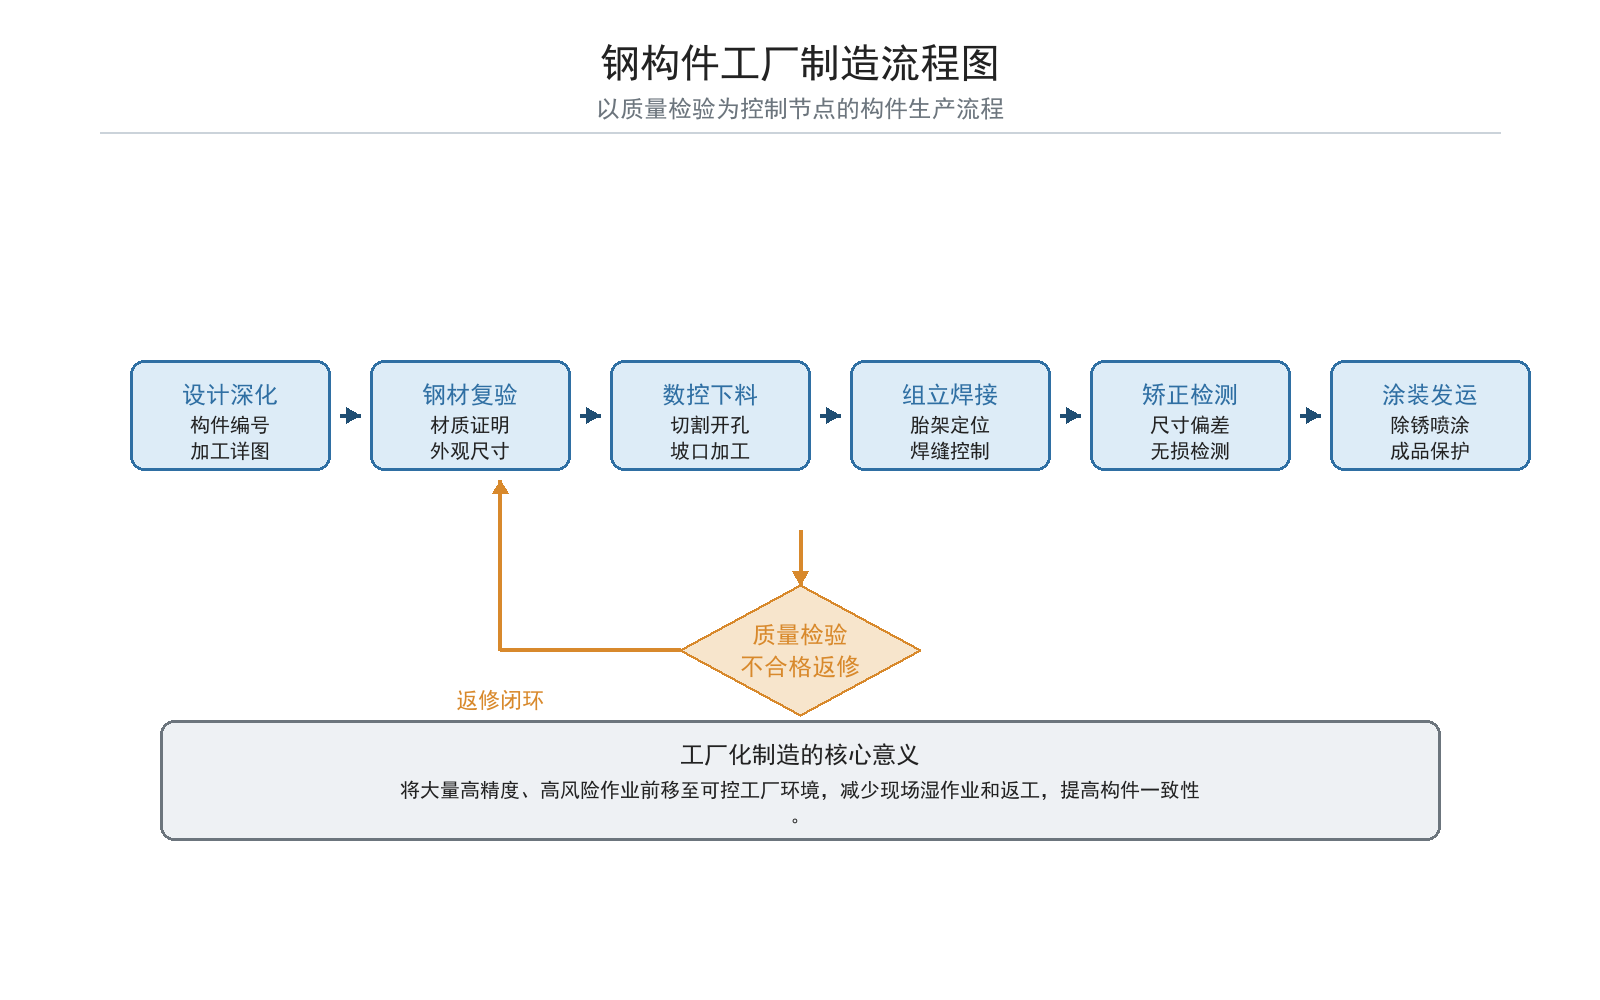
\includegraphics[width=0.92\linewidth]{figures/fig02_factory_manufacturing.png}
  \caption{钢构件工厂制造流程图}
  \label{fig:02-factory-manufacturing}
\end{figure}

% 图3：现场吊装与装配施工流程图
% 建议插入章节：关键施工技术
% 正文引用提示：如图~\ref{fig:03-site-assembly} 所示，用于说明现场装配施工从基础复核到节点验收的主要流程。
\begin{figure}[htbp]
  \centering
  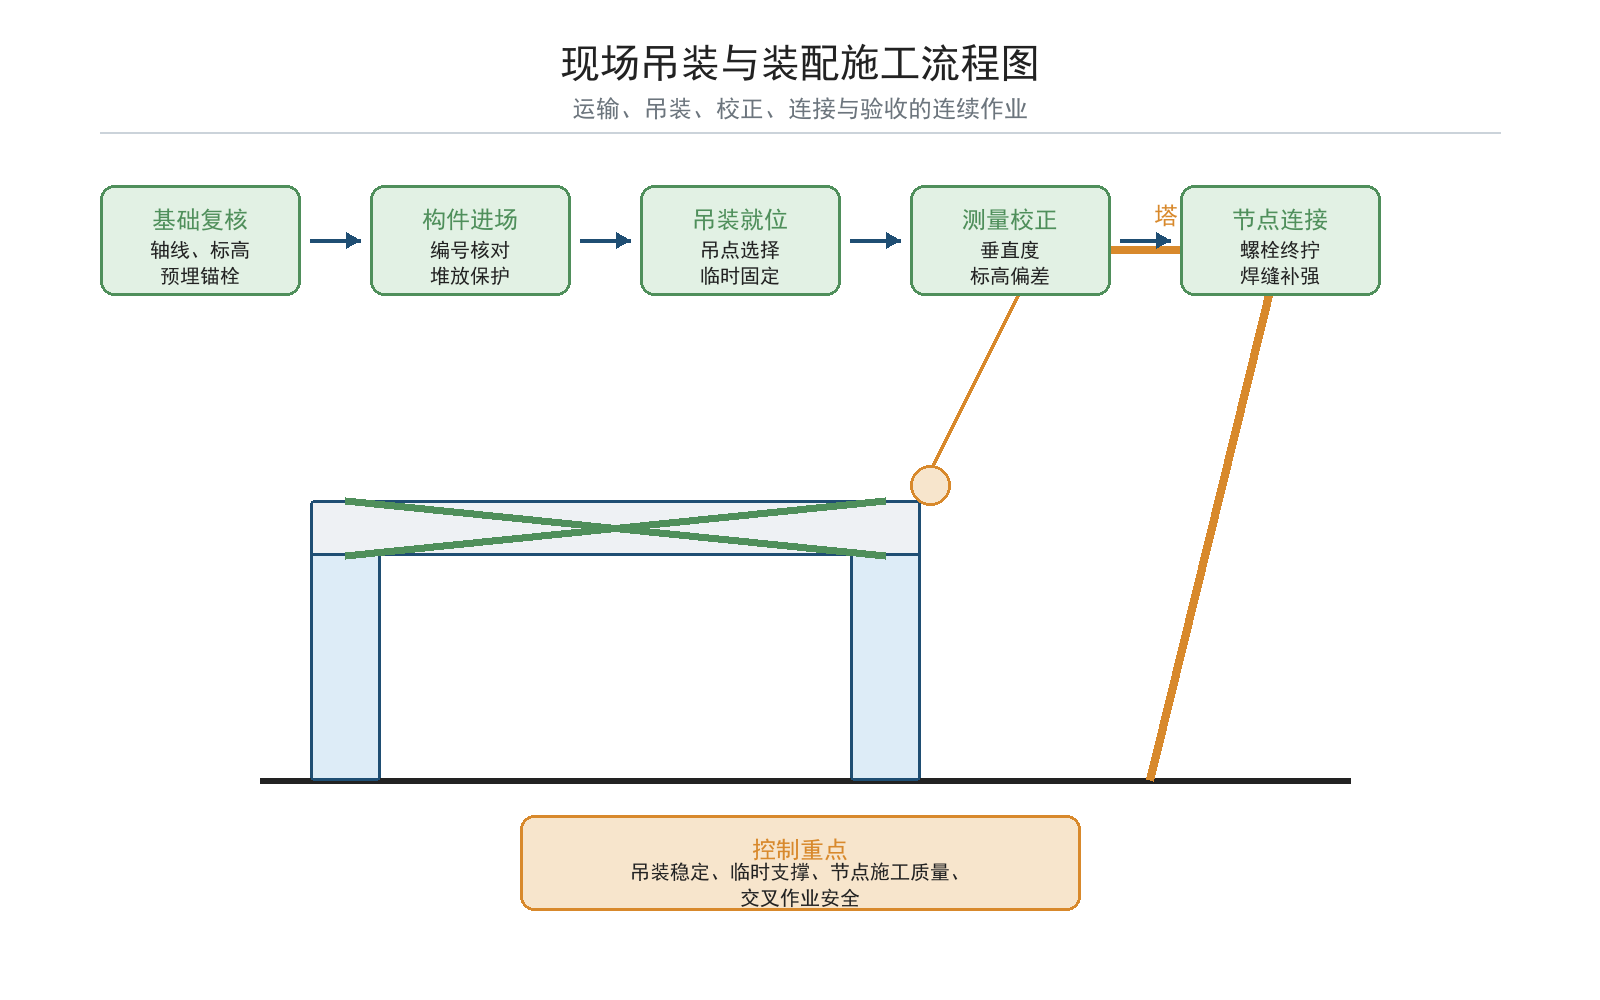
\includegraphics[width=0.92\linewidth]{figures/fig03_site_assembly.png}
  \caption{现场吊装与装配施工流程图}
  \label{fig:03-site-assembly}
\end{figure}

% 图4：梁柱螺栓连接节点示意图
% 建议插入章节：关键施工技术
% 正文引用提示：如图~\ref{fig:04-beam-column-joint} 所示，用于说明装配式钢结构常见梁柱节点的构造组成和质量控制点。
\begin{figure}[htbp]
  \centering
  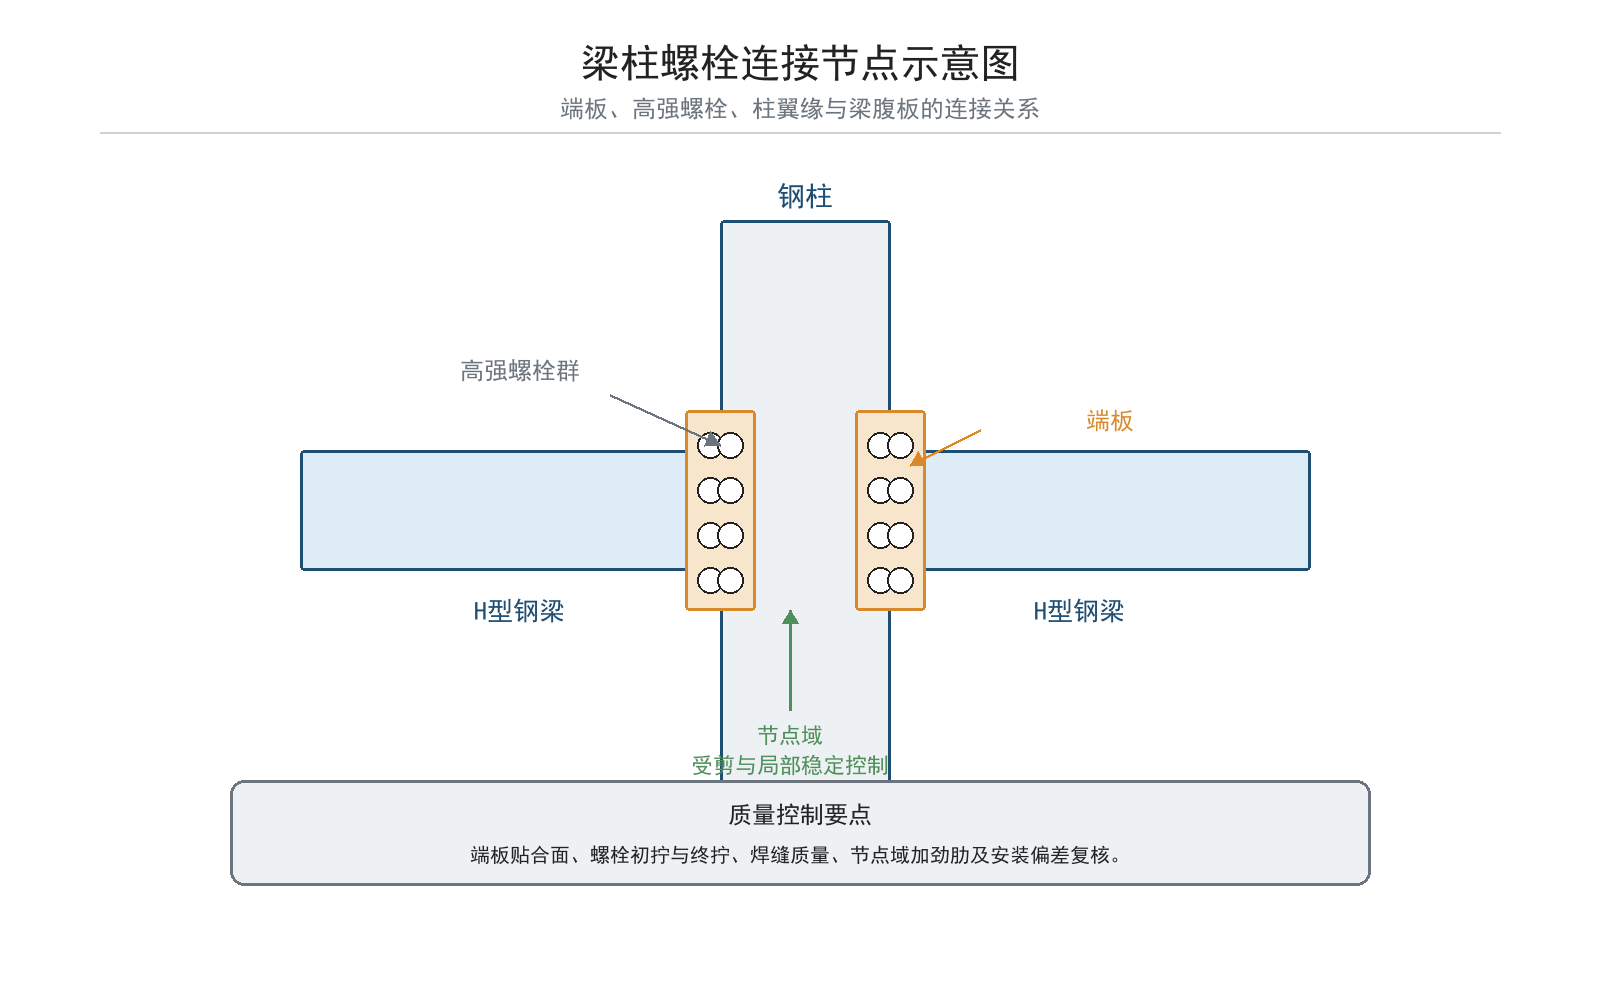
\includegraphics[width=0.92\linewidth]{figures/fig04_beam_column_joint.png}
  \caption{梁柱螺栓连接节点示意图}
  \label{fig:04-beam-column-joint}
\end{figure}

% 图5：钢框架-支撑结构受力路径示意图
% 建议插入章节：结构体系分析
% 正文引用提示：如图~\ref{fig:05-force-path} 所示，用于说明竖向荷载和水平作用在框架-支撑体系中的传递路径。
\begin{figure}[htbp]
  \centering
  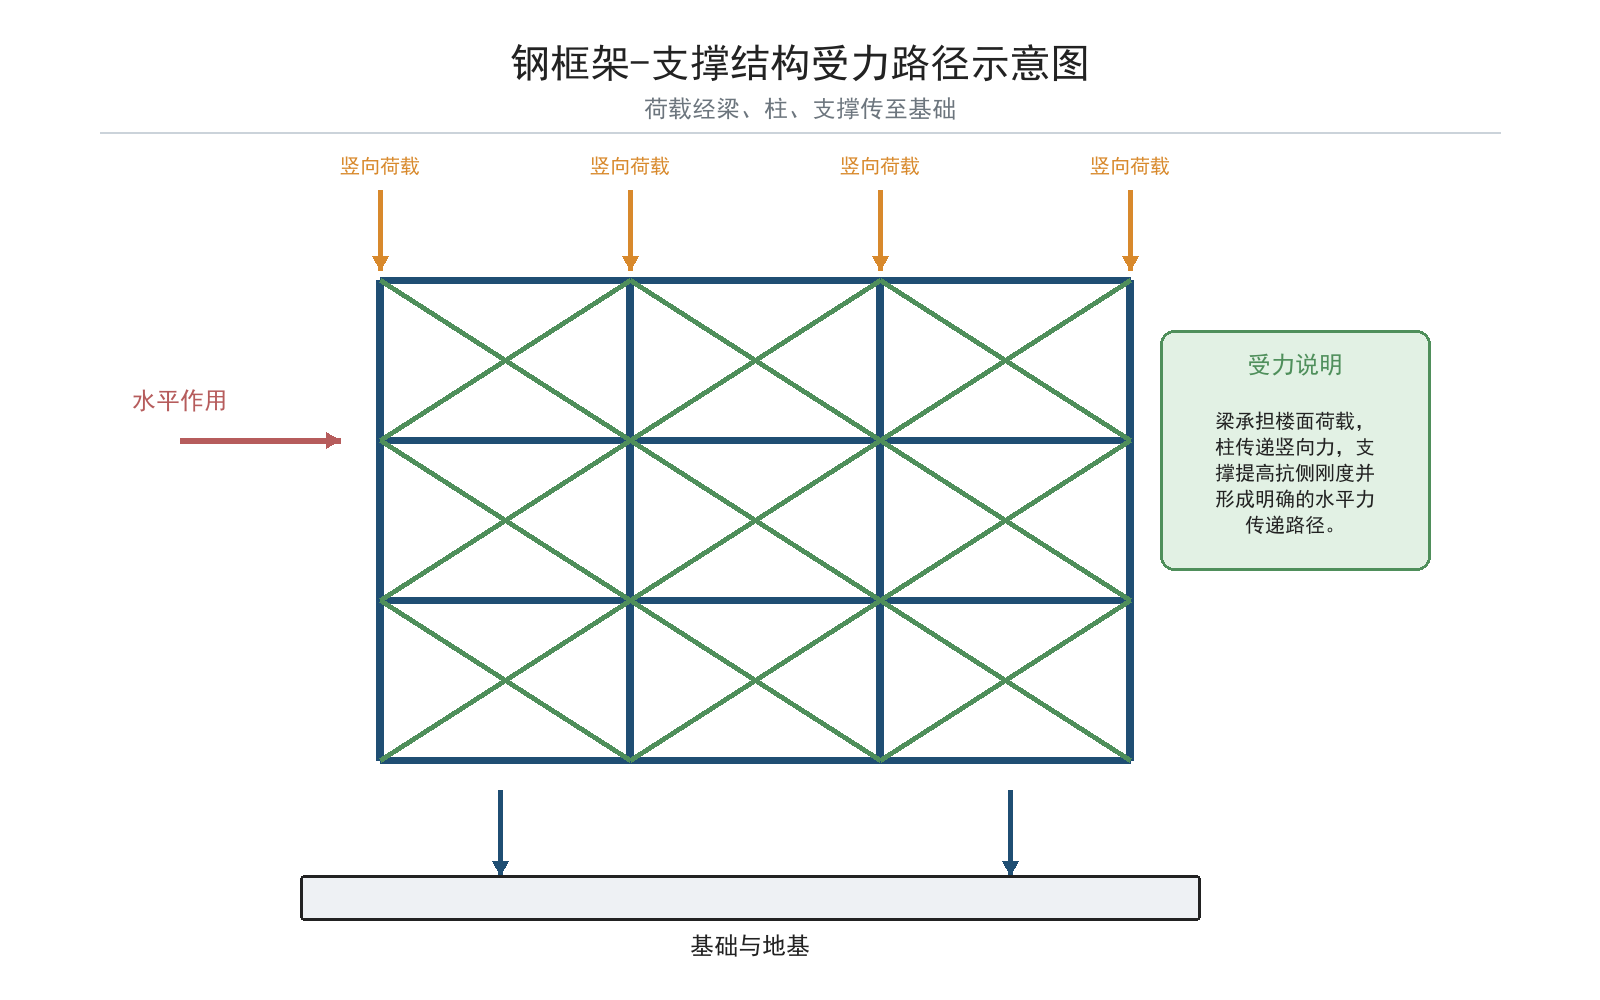
\includegraphics[width=0.92\linewidth]{figures/fig05_force_path.png}
  \caption{钢框架-支撑结构受力路径示意图}
  \label{fig:05-force-path}
\end{figure}

% 图6：楼承板组合楼盖构造示意图
% 建议插入章节：关键施工技术
% 正文引用提示：如图~\ref{fig:06-composite-floor} 所示，用于说明压型钢板、混凝土、栓钉和钢梁共同工作的组合楼盖构造。
\begin{figure}[htbp]
  \centering
  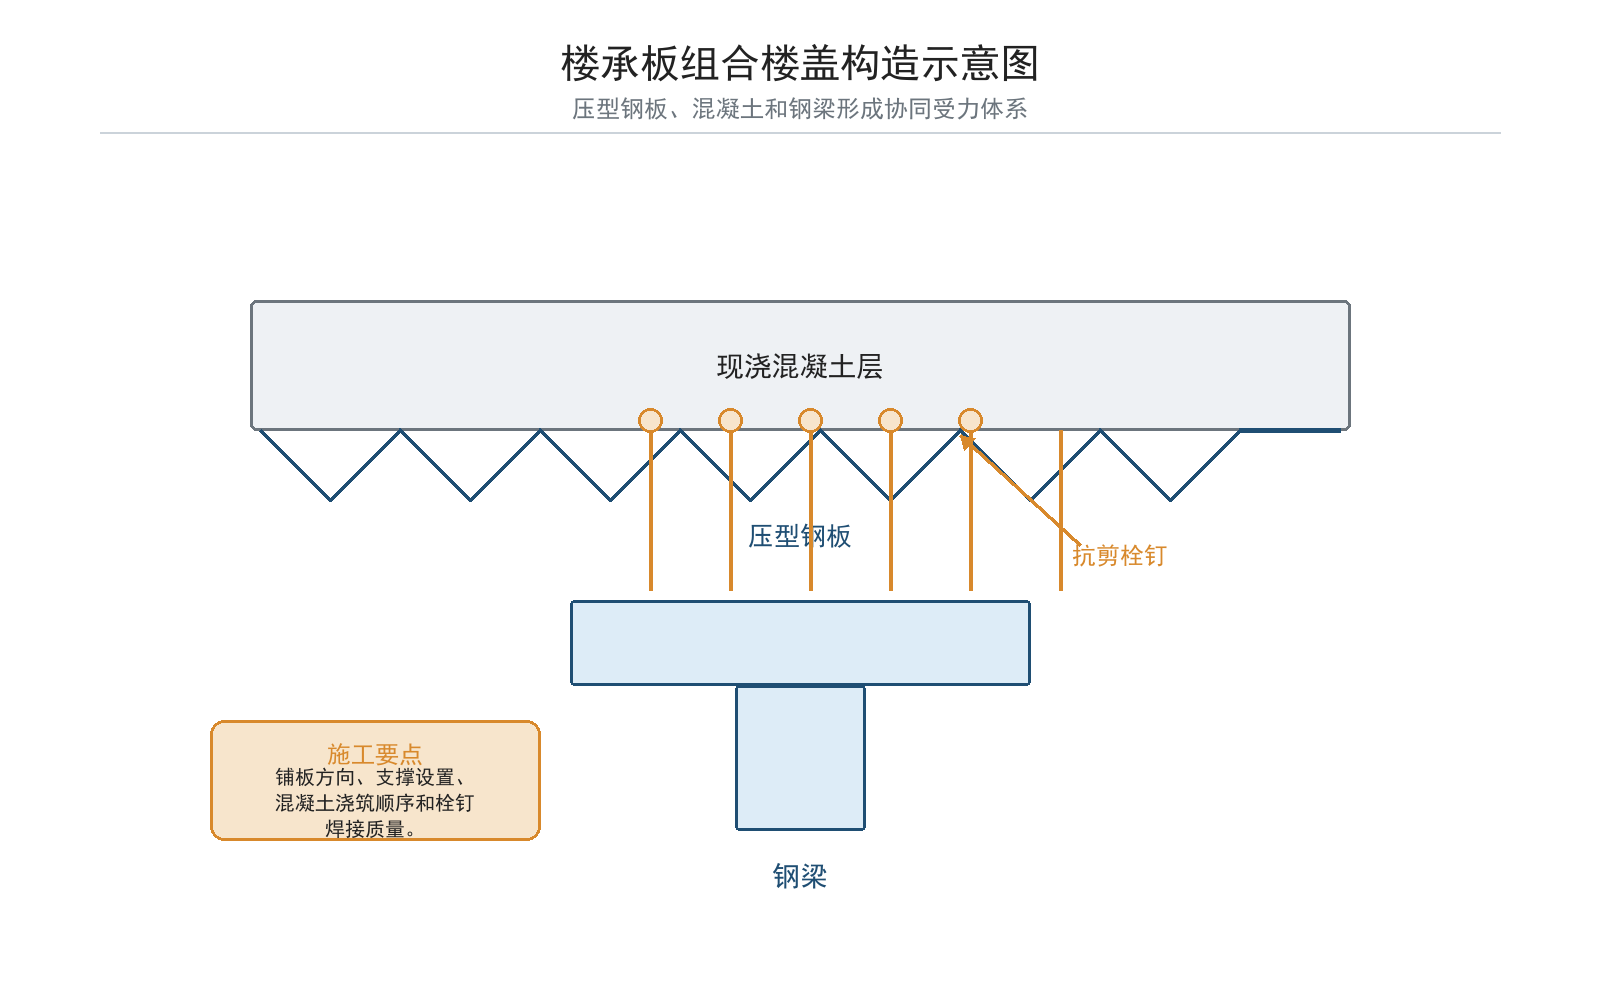
\includegraphics[width=0.92\linewidth]{figures/fig06_composite_floor.png}
  \caption{楼承板组合楼盖构造示意图}
  \label{fig:06-composite-floor}
\end{figure}

% 图7：钢结构防火保护构造示意图
% 建议插入章节：防火防腐技术
% 正文引用提示：如图~\ref{fig:07-fire-protection} 所示，用于说明钢构件外包防火涂料或板材后延缓升温的构造原理。
\begin{figure}[htbp]
  \centering
  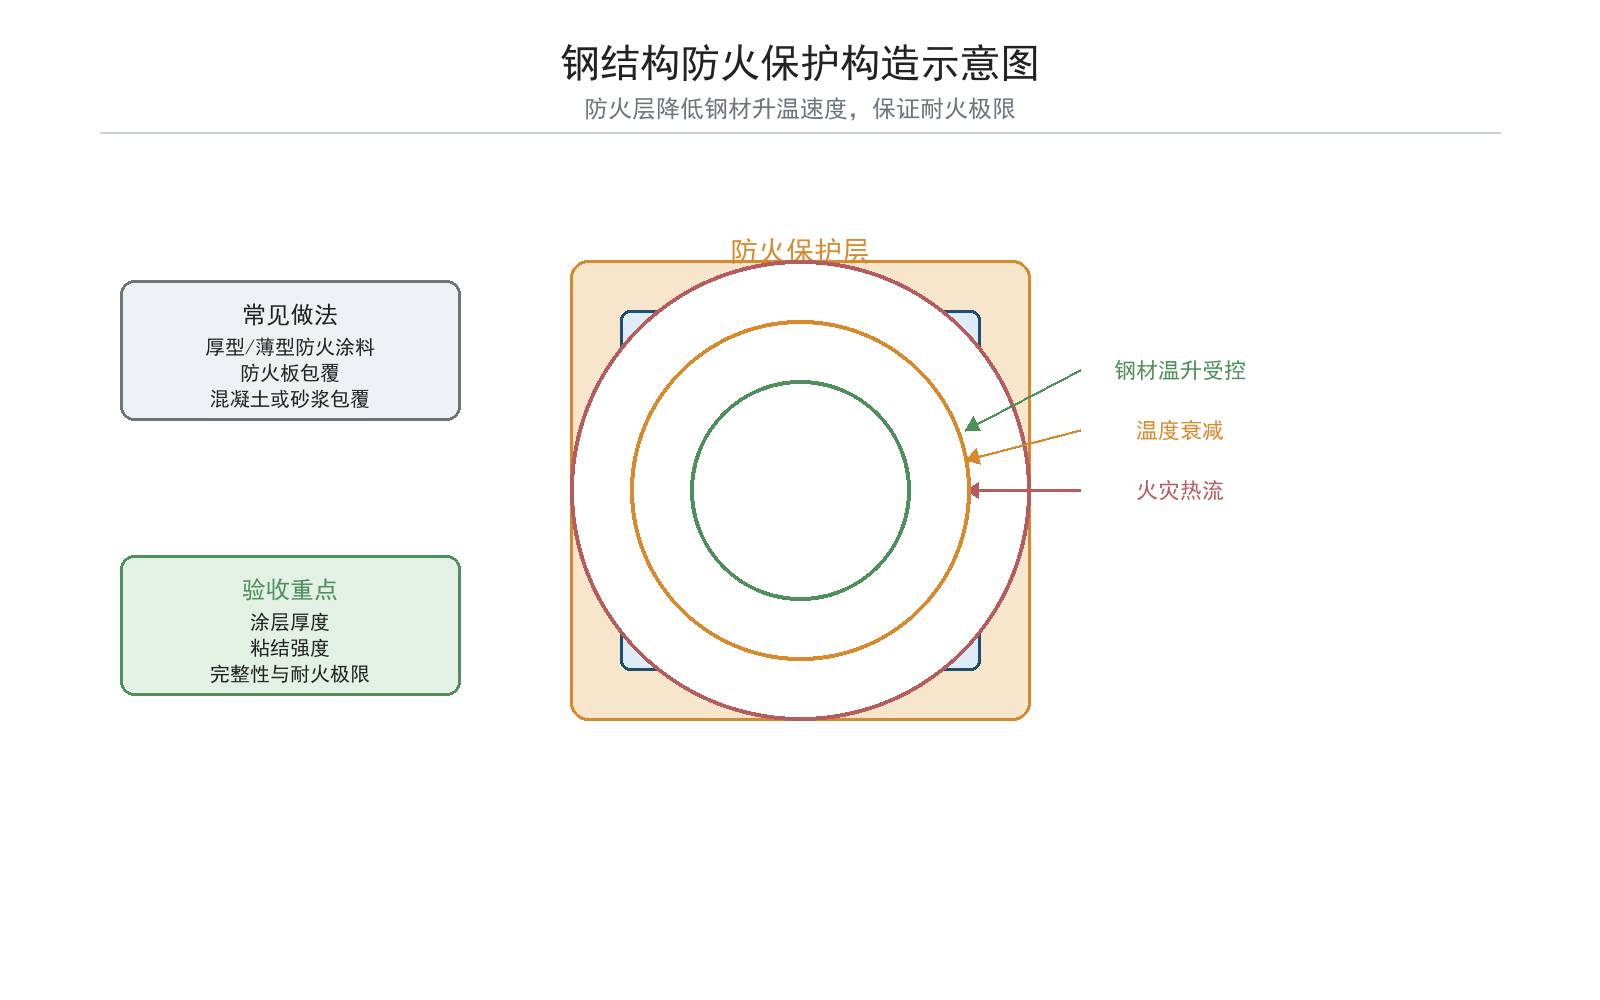
\includegraphics[width=0.92\linewidth]{figures/fig07_fire_protection.png}
  \caption{钢结构防火保护构造示意图}
  \label{fig:07-fire-protection}
\end{figure}

% 图8：钢结构防腐涂装层次示意图
% 建议插入章节：防火防腐技术
% 正文引用提示：如图~\ref{fig:08-anticorrosion-layers} 所示，用于说明钢结构防腐涂装从基层处理到面漆保护的多层体系。
\begin{figure}[htbp]
  \centering
  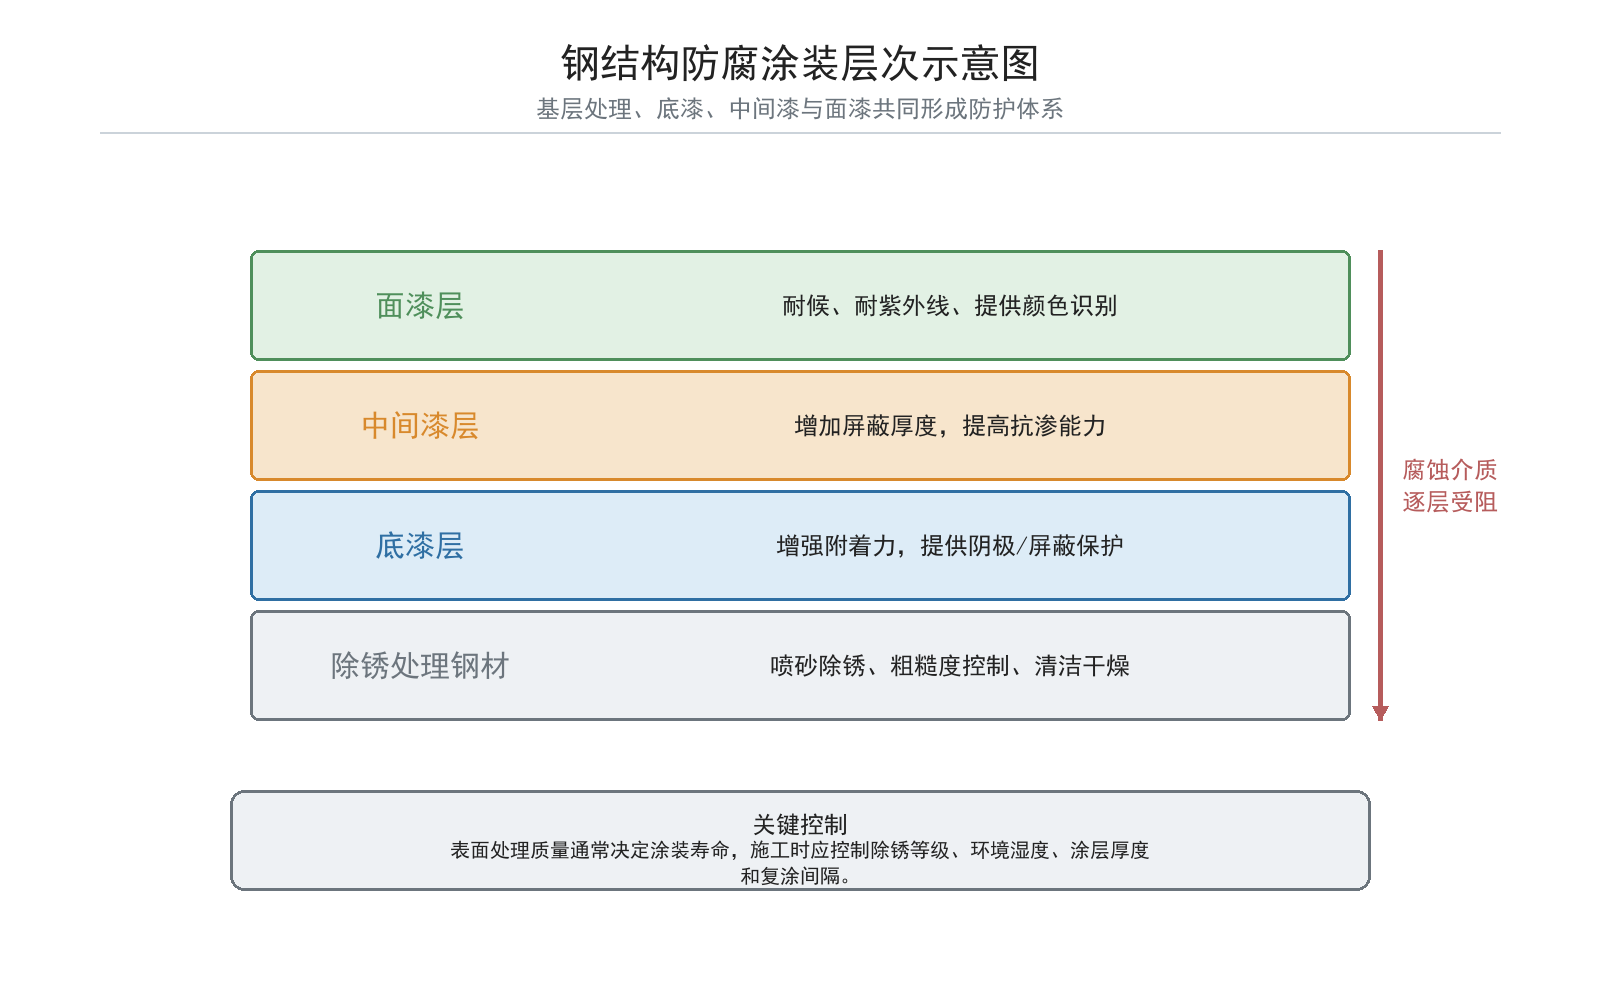
\includegraphics[width=0.92\linewidth]{figures/fig08_anticorrosion_layers.png}
  \caption{钢结构防腐涂装层次示意图}
  \label{fig:08-anticorrosion-layers}
\end{figure}

% 图9：BIM协同设计、制造、施工流程图
% 建议插入章节：发展趋势
% 正文引用提示：如图~\ref{fig:09-bim-collaboration} 所示，用于说明BIM模型在深化设计、构件加工和现场施工之间的信息传递作用。
\begin{figure}[htbp]
  \centering
  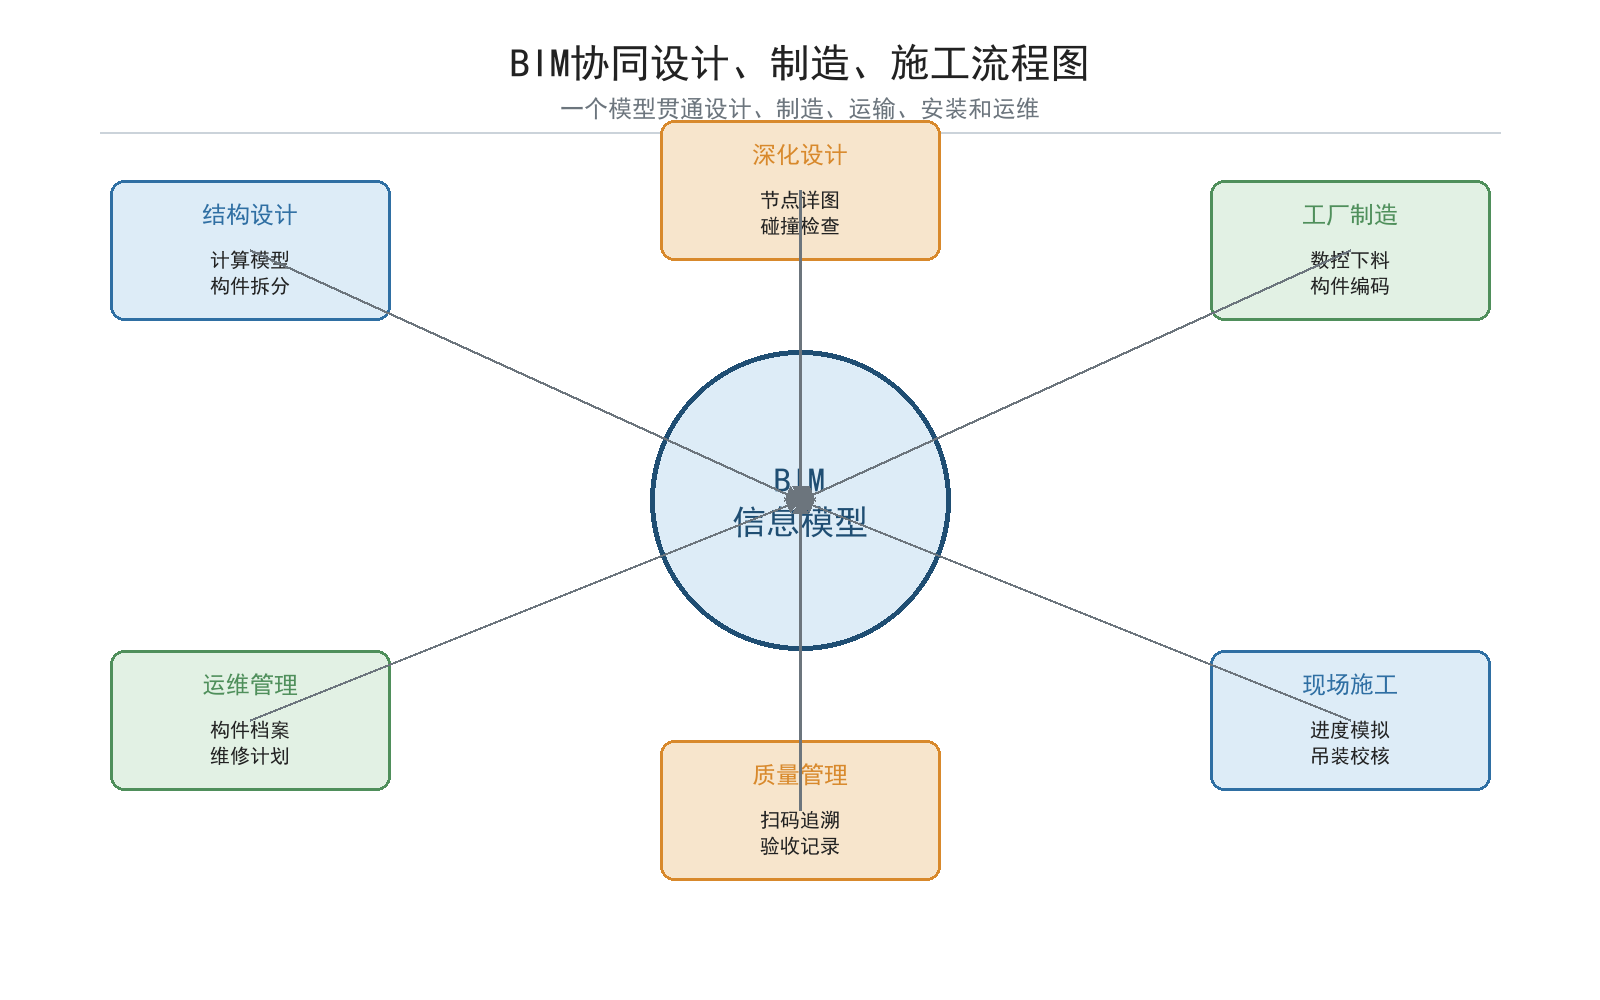
\includegraphics[width=0.92\linewidth]{figures/fig09_bim_collaboration.png}
  \caption{BIM协同设计、制造、施工流程图}
  \label{fig:09-bim-collaboration}
\end{figure}

% 图10：装配式钢结构质量控制闭环图
% 建议插入章节：应用问题与质量控制
% 正文引用提示：如图~\ref{fig:10-quality-control-loop} 所示，用于说明质量控制应覆盖设计、制造、运输、安装和验收反馈全过程。
\begin{figure}[htbp]
  \centering
  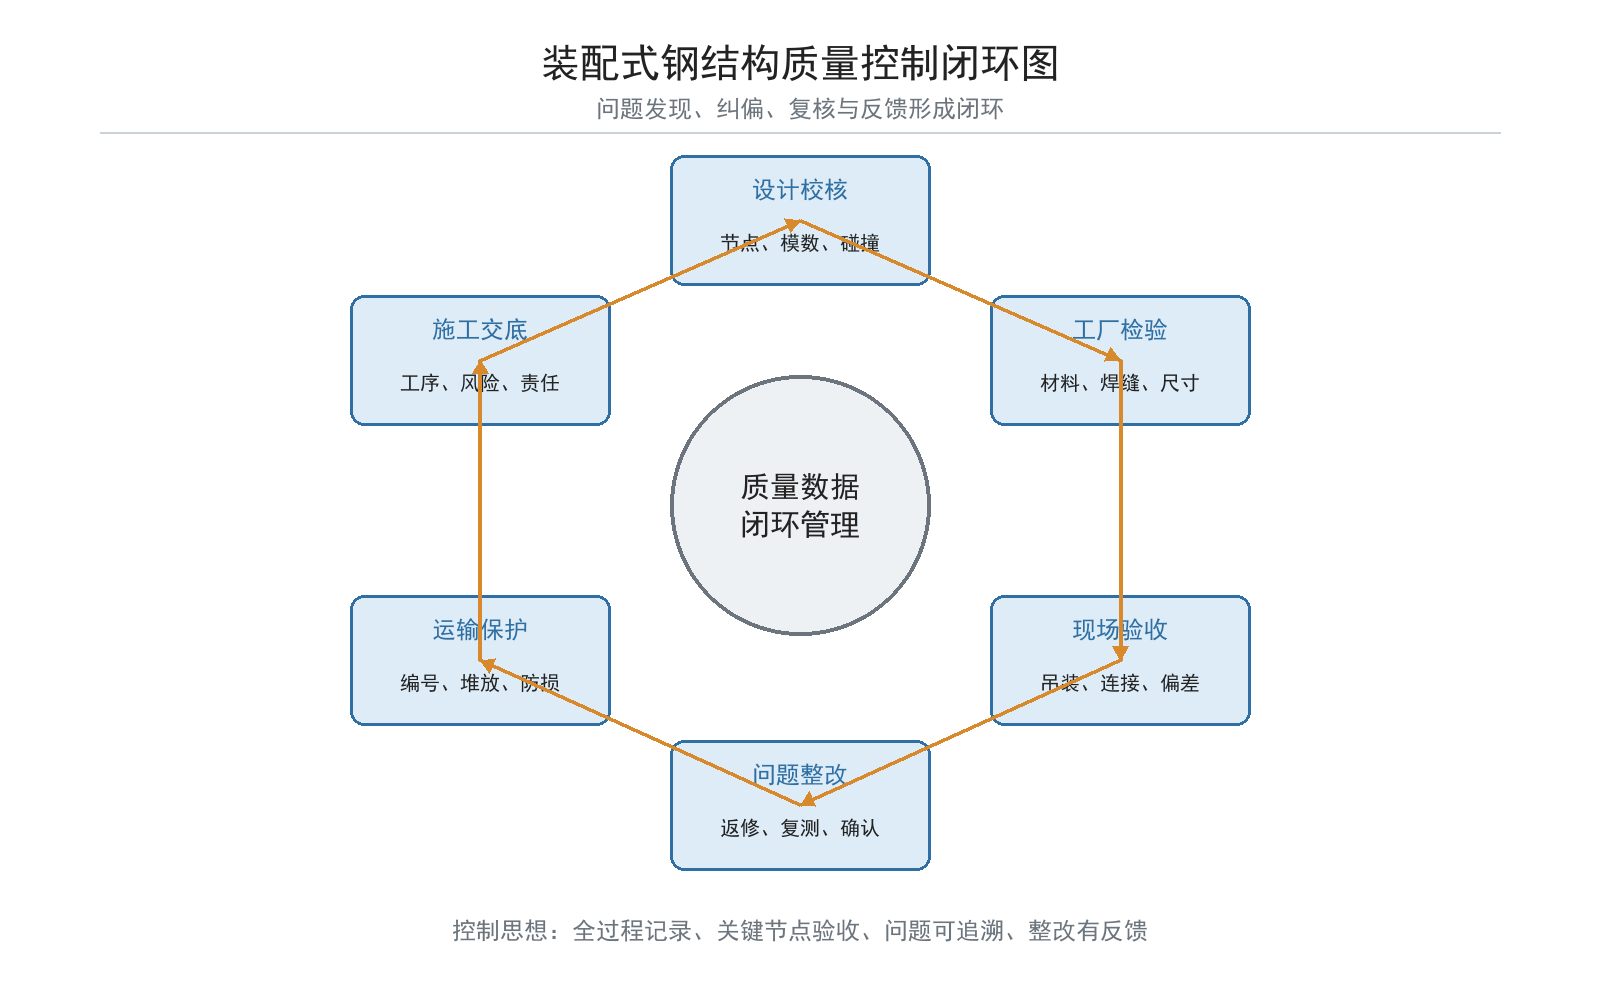
\includegraphics[width=0.92\linewidth]{figures/fig10_quality_control_loop.png}
  \caption{装配式钢结构质量控制闭环图}
  \label{fig:10-quality-control-loop}
\end{figure}

% 图11：装配式钢结构绿色建造优势示意图
% 建议插入章节：发展背景或发展趋势
% 正文引用提示：如图~\ref{fig:11-green-construction} 所示，用于说明钢结构装配化在节材、节水、减排和可回收方面的综合优势。
\begin{figure}[htbp]
  \centering
  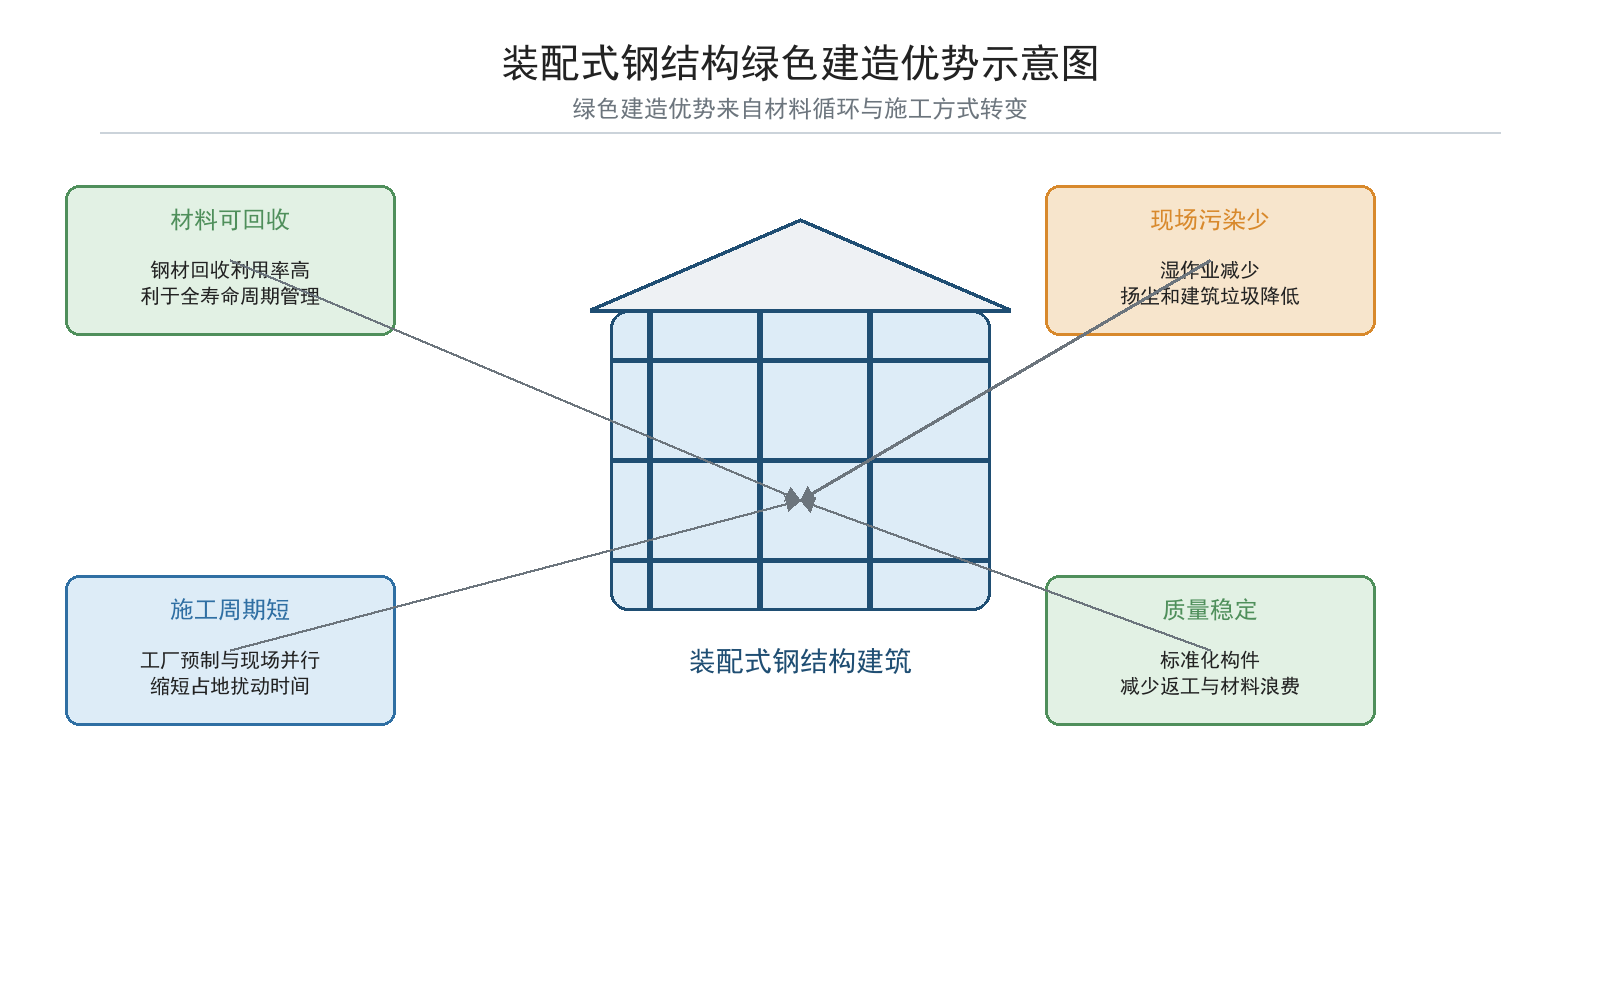
\includegraphics[width=0.92\linewidth]{figures/fig11_green_construction.png}
  \caption{装配式钢结构绿色建造优势示意图}
  \label{fig:11-green-construction}
\end{figure}

% 图12：装配式钢结构未来发展趋势路线图
% 建议插入章节：发展趋势
% 正文引用提示：如图~\ref{fig:12-development-roadmap} 所示，用于概括装配式钢结构从标准化到智能化、低碳化的发展方向。
\begin{figure}[htbp]
  \centering
  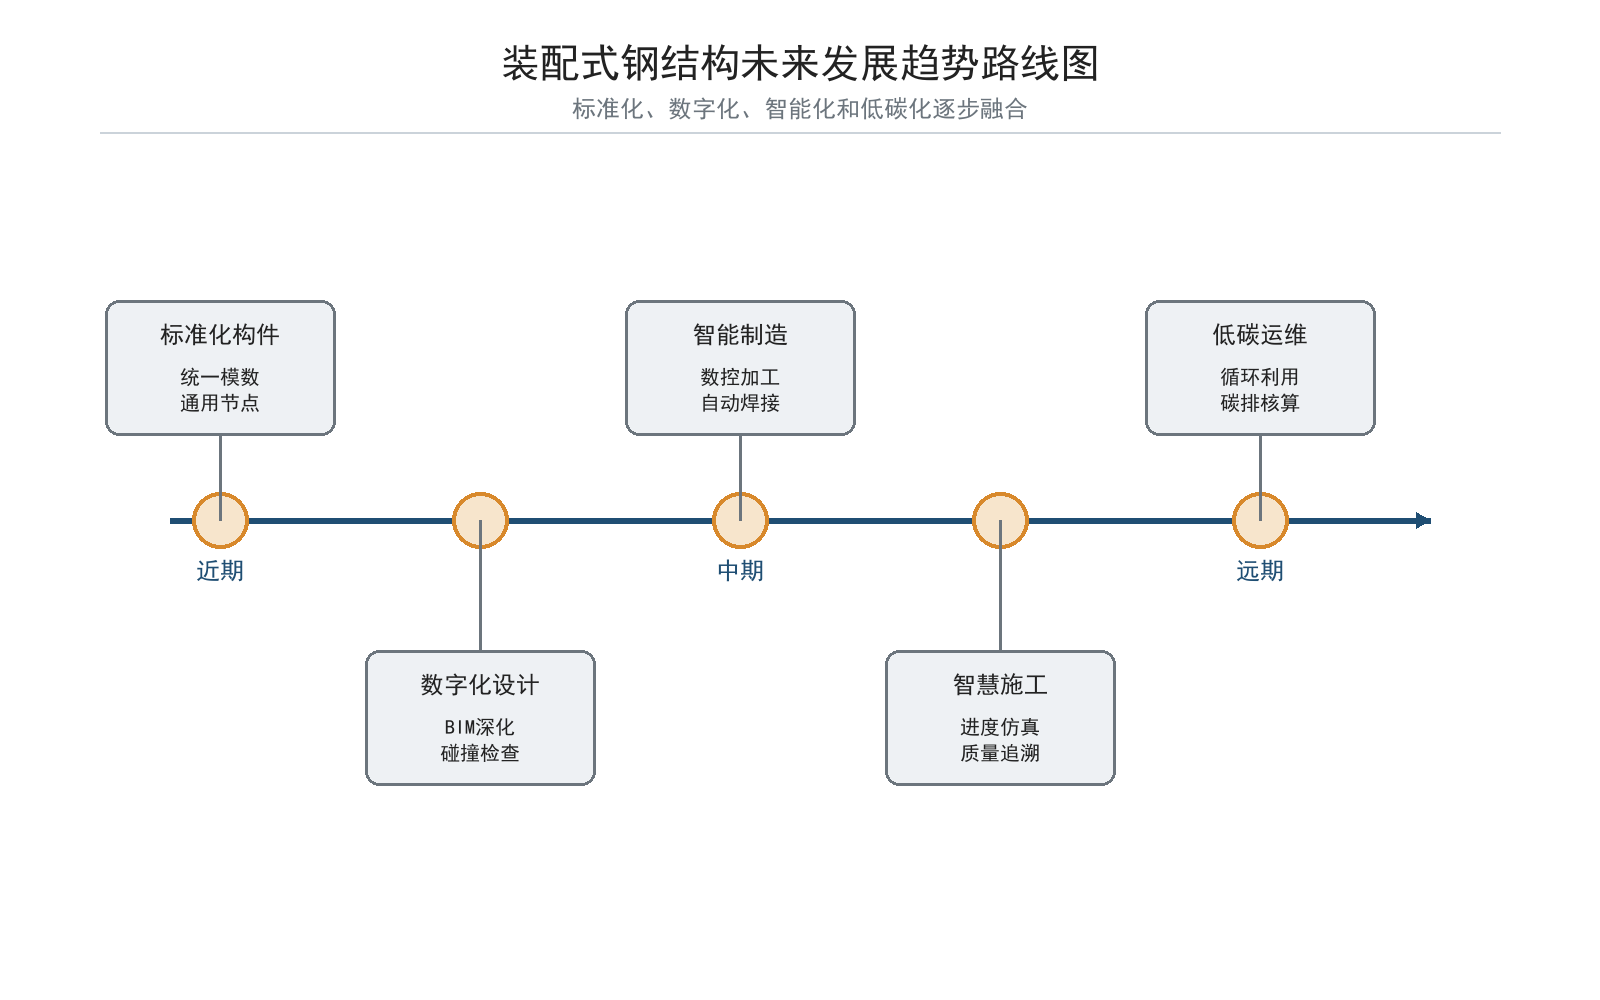
\includegraphics[width=0.92\linewidth]{figures/fig12_development_roadmap.png}
  \caption{装配式钢结构未来发展趋势路线图}
  \label{fig:12-development-roadmap}
\end{figure}

% 图13：传统现浇建筑与装配式钢结构施工流程对比图
% 建议插入章节：应用问题或技术特点
% 正文引用提示：如图~\ref{fig:13-process-comparison} 所示，用于对比传统现浇模式与装配式钢结构在流程组织上的差异。
\begin{figure}[htbp]
  \centering
  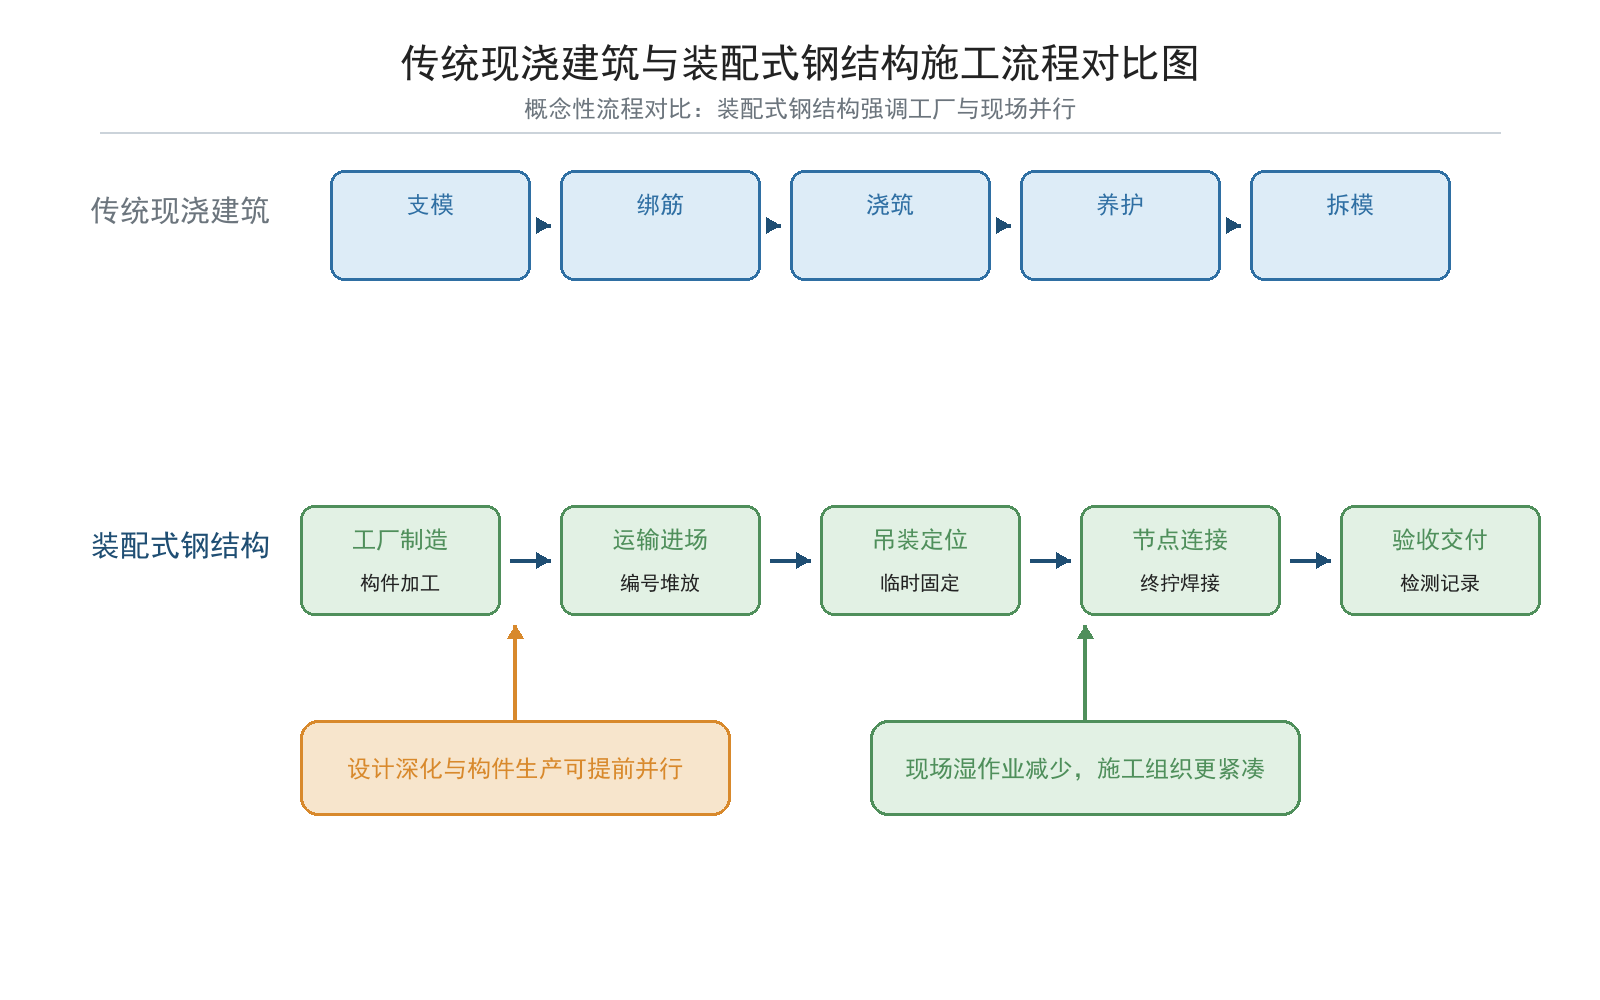
\includegraphics[width=0.92\linewidth]{figures/fig13_process_comparison.png}
  \caption{传统现浇建筑与装配式钢结构施工流程对比图}
  \label{fig:13-process-comparison}
\end{figure}

% 图14：钢结构、混凝土结构、木结构综合特点对比雷达图
% 建议插入章节：技术特点
% 正文引用提示：如图~\ref{fig:14-structure-radar} 所示，概念性对比图，用于展示三类结构在若干性能维度上的相对特点。
\begin{figure}[htbp]
  \centering
  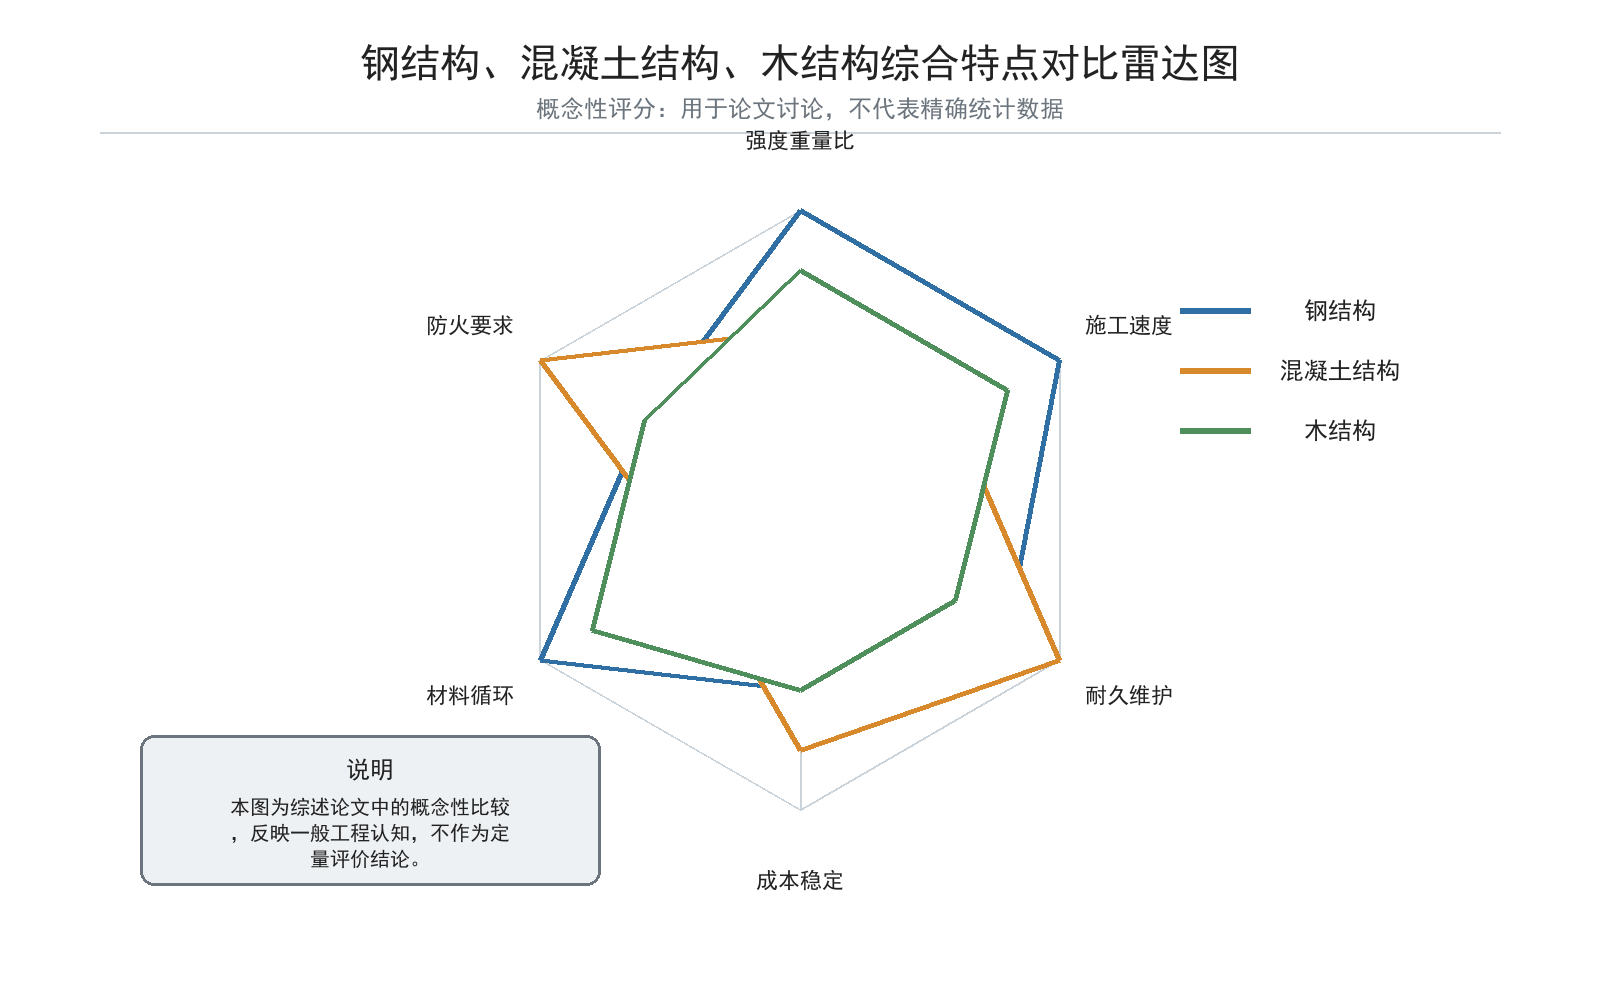
\includegraphics[width=0.92\linewidth]{figures/fig14_structure_radar.png}
  \caption{钢结构、混凝土结构、木结构综合特点对比雷达图}
  \label{fig:14-structure-radar}
\end{figure}

% 图15：装配式钢结构推广影响因素权重示意图
% 建议插入章节：应用问题
% 正文引用提示：如图~\ref{fig:15-adoption-factors} 所示，概念性权重图，用于归纳影响装配式钢结构推广的主要因素。
\begin{figure}[htbp]
  \centering
  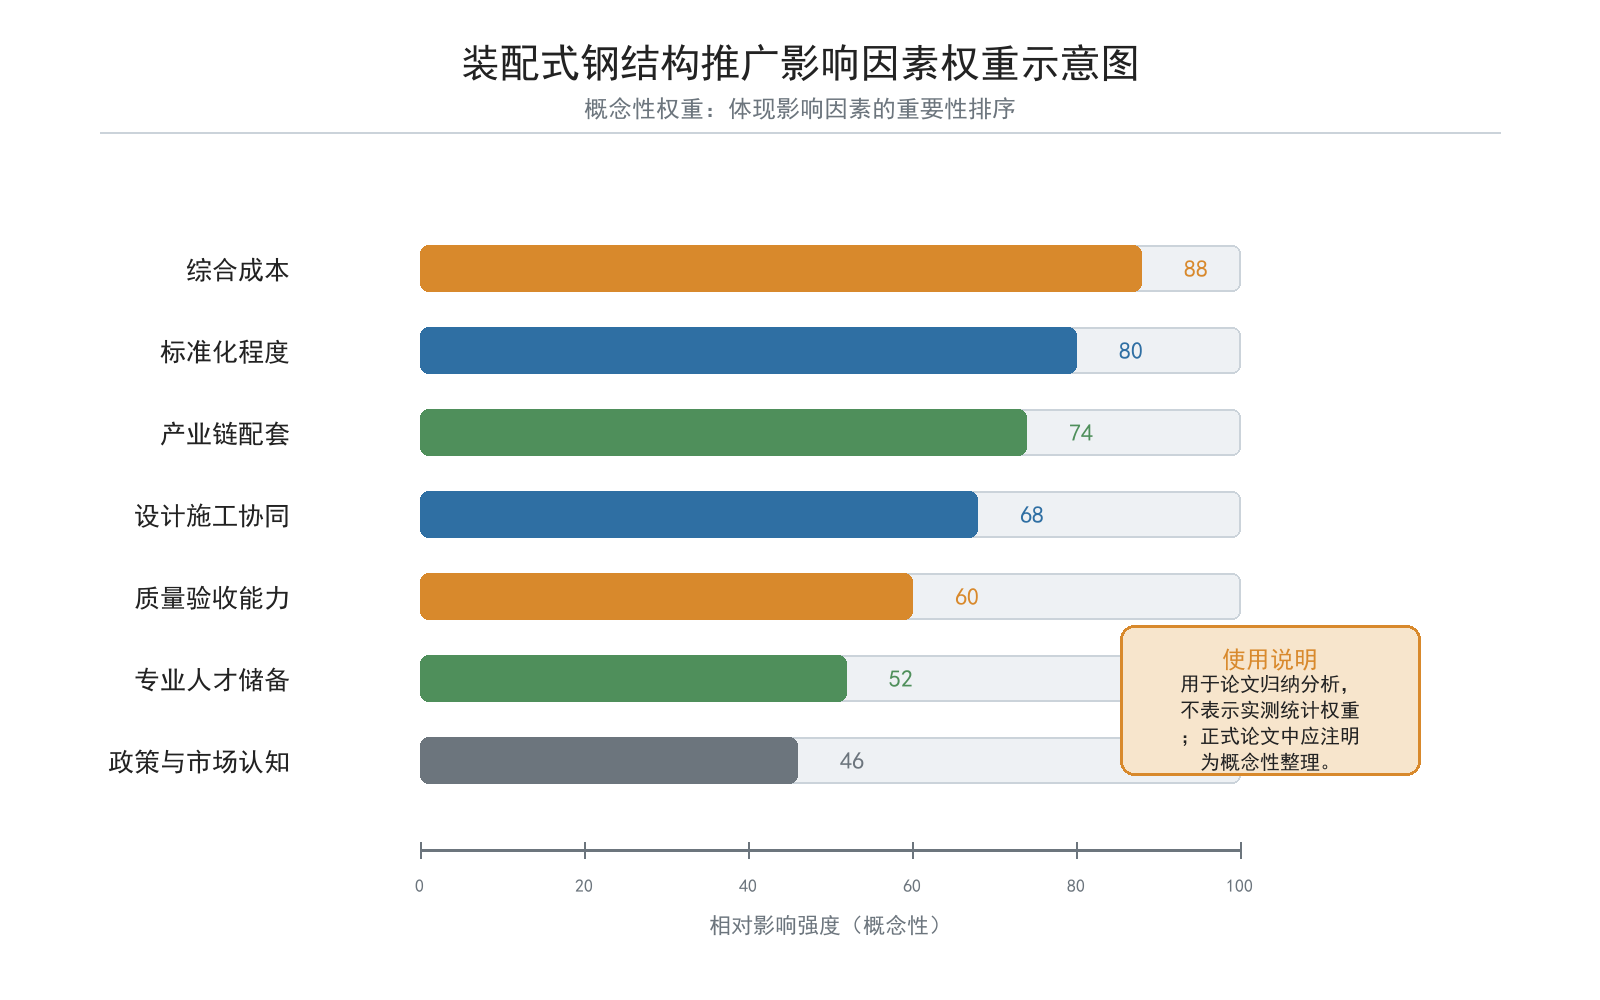
\includegraphics[width=0.92\linewidth]{figures/fig15_adoption_factors.png}
  \caption{装配式钢结构推广影响因素权重示意图}
  \label{fig:15-adoption-factors}
\end{figure}
